\chapter{Project description}
This chapter provides an overall description of the project including a brief overview of the main technologies used.

The overall topic of the R\&D project is source-code generation, which derives from automatic programming. Automatic programming can be defined as the automation of some part of the programming process \cite{barrAutomaticProgramming1982}. The process consists of parsing a specification as an input to the automatic programming system which outputs a program \cite{novakjr.CS394PAutomatic}.\\
An example of an automatic programming system could be a compiler, where the specification is a program written in the desired programming language and the output is an executable program. Another example could be the tools provided by Visual Paradigm that translates the contents of UML diagrams to source-code of different programming languages \cite{visualparadigmUMLCodeGeneration}.\\
The motivation behind automatic programming is that it allows developers to express themselves more abstractly through specifications, allowing for smaller, more understandable and less error-prone programs \cite{novakjr.CS394PAutomatic}.

Source-code generation can be considered a specific area of automatic programming where the output of the automatic programming system is source-code. 
The motivation for source-code generation is similar to that of automatic programming, however, the output is a refined or generated specification rather than an executable program.

This R\&D project investigates the usage of the library LibTooling for writing deterministic C++ source-code generation tools. The project involves the writing of three separate tools with increasing complexity that addresses some issues related to writing source-code generation tools through LibTooling.

The first tool is a simple renaming tool that can be used to rename functions and their matching invocations.\\
The second tool is also a refactoring tool which transforms arrays specified using the C-style notation into the more modern and secure \cppinline{std::array} notation. \\
The third tool generates a \cppinline{to_string} function for each enum declaration inside the program, i.e., a function that takes an instance of that enum as an argument and returns a string corresponding to the name of the value of the enum. If an existing \cppinline{to_string} function exists, e.g., in another namespace, the tool updates it in place instead.

\section{Technology overview}
The LLVM project is a collection of compiler and toolchain technologies that can be used to build compiler-frontends for programming languages and compiler-backends for multiple instruction set architectures \cite{llvmLLVMCompilerInfrastructure}.
One project created alongside LLVM is Clang. Clang is a compiler-frontend for languages in the C language family including C, C++, Objective C and many others \cite{clangClangLanguageFamily}.\\
The LibTooling library was created as part of the Clang project and it allows developers to build standalone tools based on Clang \cite{llvmLibToolingClang17}. 
The library provides access to Clang's AST parser and LLVM's command line parsing. As C++ is a complex programming language with context-sensitive grammar, having access to an existing parser through the library is a great starting point for tool development \cite{swarnimProblemsPainsParsing}. The library APIs hook into the compilation pipeline after the parsing step, which guarantees that the tool is only run on valid AST. Furthermore, Clangs AST is very fine-grained allowing for a detailed analysis of the provided source-code, which is very helpful when developing tools \cite{clangIntroductionClangAST}. The full compilation pipeline of Clang and LLVM can be seen on \cref{fig:040des:llvmToolchainOverview}. The structure of a tool created with LibTooling can be seen on \cref{fig:040des:clangToolingOverview}.

\begin{figure}[H]
    \centering
    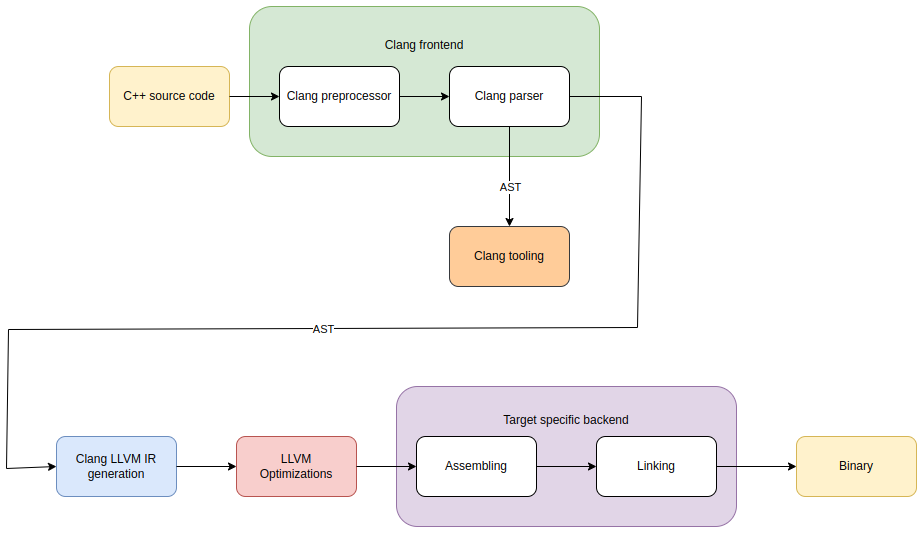
\includegraphics[width=0.9\textwidth]{figs/040des/compilation_overview.png}
    \caption{Overview of the Clang and LLVM compilation pipeline. The yellow blocks in the diagram are in/outputs of the pipeline. The green box is the Clang frontend. The blue box is the conversion step between the Clang frontend and the LLVM backend. The red box is the LLVM optimizations. The purple box represents the tasks of the backend for the specific instruction set architecture.}
    \label{fig:040des:llvmToolchainOverview}
\end{figure}

\begin{figure}[H]
    \centering
    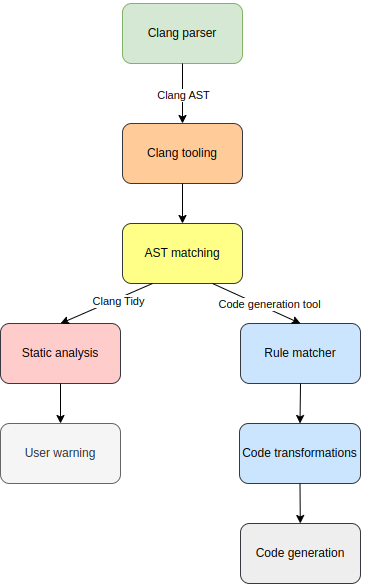
\includegraphics[width=0.4\textwidth]{figs/040des/clang_tool_pipeline.png}
    \caption{An overview of the Clang frontend and the LibTooling library. The green and orange boxes are identical to the boxes in \cref{fig:040des:llvmToolchainOverview}. The yellow box is the filtering/semantic analysis of the AST for the given tool. The tree splits into two to show that multiple different tools can use the library. On the left with the red box is the structure of the popular Clang-tidy tool\cite{clangClangTidyExtraClang}. On the right in blue is the structure of a custom tool as developed in this project. The two grey boxes indicate outputs from the tools.}
    \label{fig:040des:clangToolingOverview}
\end{figure}


\section{Project delimitations}
While LibTooling supports writing tools for programming languages in the C language family, this project is delimited to focusing on tools written for C++.

In many cases, it may be beneficial to integrate the tools developed with LibTooling into the development flow by providing it as a Clang plugin.
While the project will not delve into this topic, it is worth mentioning that the developed tools have the potential to be exported as Clang plugins \cite{clangClangPluginsClang}.

At last, LibTooling offers multiple APIs for developing standalone tools. Although the APIs may have different appearances, they essentially provide similar functionality. They can all be utilized to develop tools that leverage the Clang AST but adopt different software patterns in doing so.
A few examples of the APIs are RecursiveASTVisitor, LibASTMatchers and Clang Transformer \cite{clangHowWriteRecursiveASTVisitor,clangWelcomeClangDocumentation}. This project will focus on the Clang Transformer API and, as a result, will not go into detail about the alternative APIs in LibTooling \cite{clangClangTransformerTutorial}.

\section{Methods}
As described earlier three different tools were developed during the project. The tools are used as a progressive learning platform for exploring increasingly complex parts of the LibTooling library. 

The first tool is a renaming tool, that will refactor a method with an illegal name (``MkX'') into a legal name (``MakeX''). The tool will also rename all the calls to the renamed method to keep the specification valid. The purpose of developing this tool is to get familiar with the basics of the LibTooling library, which will make later development easier. 

The second tool is also a refactoring tool but with more complexity than the renaming tool. The purpose of the second tool is to convert traditional C-style arrays into the more modern and strongly typed \cppinline{std::array}s. This tool is more complex than the renaming tool because there is more information associated with arrays than function names. Furthermore, there are more semantic considerations which have to be taken into account when making this type of change.
Developing this tool brings insight into the challenges related to automatically refactoring more complex declarations.

The third tool analyzes the code base for enum declarations and generates ``to\_string'' functions for each enum declaration. The ``to\_string'' function will return a string representation of the named enum constants defined in the enum. In order to ensure the source-code is valid after the tool is run, existing ``to\_string'' functions should be overwritten, updated or removed as a part of the process. 
This tool is comparable in complexity to the C-style converter tool but adds the complexity of code generation to the tool.
Furthermore, the tool is implemented following two different strategies in order to compare and explore different methodologies.

Through these three tools, a deeper understanding of the LibTooling library and the C++ language is obtained.